\chapter{Results}\label{ch:results}
In this section, we want to evaluate our results for the \ac{CEP} extraction algorithm, \ac{WDCG} and the overall performance of the End-to-End pipeline.


\section{Performance Of The Cause-Effect Pairs Extraction}\label{sec:performance-measure}
\begin{figure}
    \begin{center}
        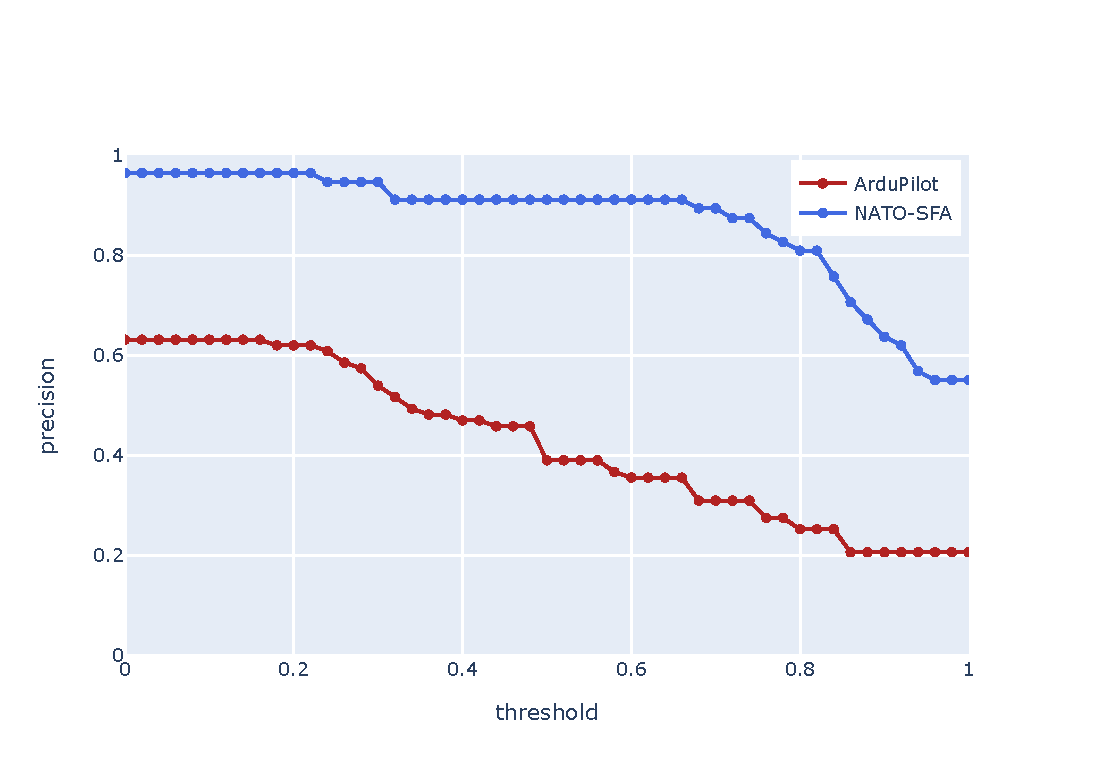
\includegraphics[scale=.65]{figures/results/precision}
        \caption{Precision comparison between ArduPilot and NATO-SFA dataset}\label{fig:precision}
        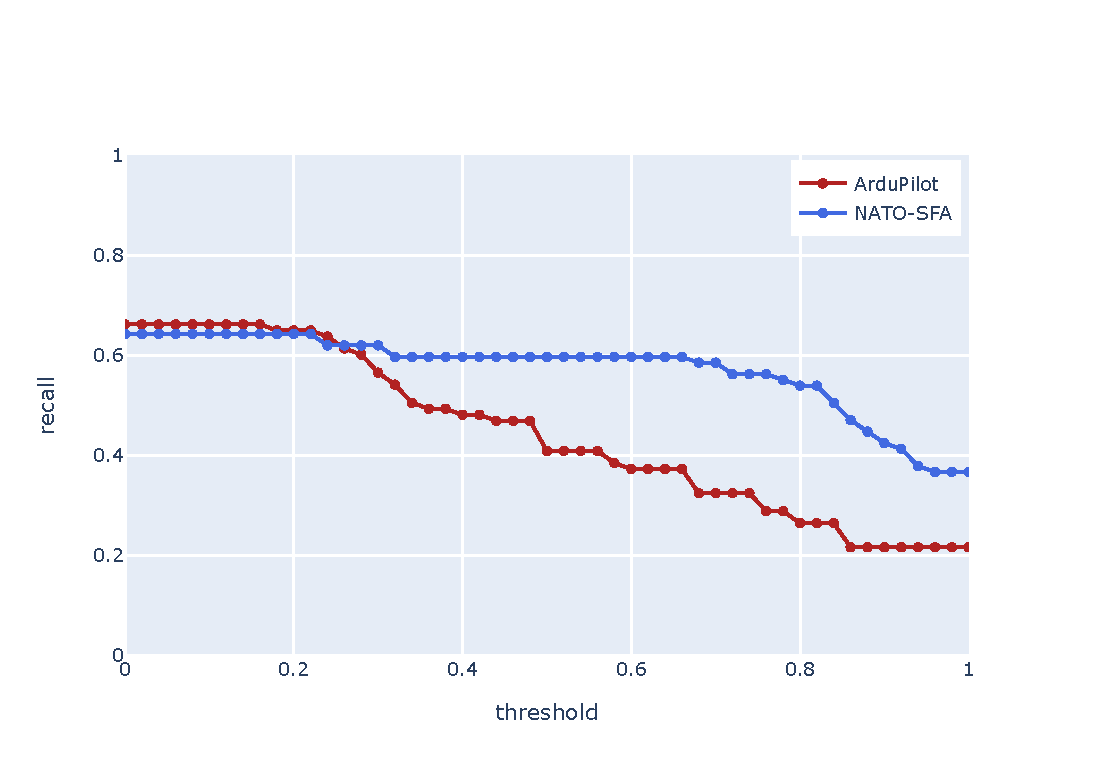
\includegraphics[scale=.65]{figures/results/recall}
        \caption{Recall comparison between ArduPilot and NATO-SFA dataset}\label{fig:recall}
    \end{center}
\end{figure}
In \autoref{fig:precision} and \autoref{fig:recall} we can see the precision and recall of the \ac{CEP} extraction algorithm for the Ardupilot dataset in comparison to the NATO-SFA benchmark dataset.
In addition, the graphs plot the performance scores based on different threshold values (see. \autoref{subsec:performance-measurement}).
We can first notice that the curves are continuously decreasing, that is because, for a higher threshold value, more \ac{CEP}s are not matching.
Thus, the \ac{FP} and \ac{FN} are increasing, which leads to this behavior.
Second, the precision score of the \ac{NATO-SFA} dataset is for each threshold value higher than the precision score of the ArduPilot dataset.
The reason for that is that the \ac{NATO-SFA} dataset consists of shorter sentences with longer phrases, which makes it more likely to hit such a phrase which leads to a \ac{TP}.
In contrast, the recall scores between the datasets are more similar, and only at a threshold value > 0.3 the \ac{NATO-SFA} dataset has a higher recall.
Recall defines how many labeled \ac{CEP}s we are hitting.
Thus, we can say that the algorithm we provide is general in detecting \ac{CEP}s.
In \autoref{fig:recall} the authors achieved with comparable dependency patterns, but without handling multiple \ac{CEP}s and conjunctions a precision of \qq{0.5083},  recall \qq{0.3566} and f1-score of \qq{0.4191}.
Furthermore, they measured these scores with strict rules for the \qq{matching} term (see \autoref{sec:measure-the-performance-of-the-cause-effect}).
This would be similar for any threshold value greater than zero with our approach.
To compare their results with ours, we use the threshold value of 0.01.
We achieved a precision \qq{0.6322}, recall \qq{0.6626} and f1 \qq{0.6471} at the ArduPilot dataset.
Thus we were able to improve the performance measurements with our approach.
Furthermore, we were able to have even a better precision for threshold vales < 0.32 and a better recall for threshold values < 0.66.
Additionally we achieved a precision \qq{0.9655}, recall \qq{0.6437} and f1 \qq{0.7724} score on the \ac{NATO-SFA} dataset.
Thus our method of extracting multiple \ac{CEP}s is well-performing.


\section{Causal Graph Evaluation}\label{sec:causal-graph-evaluation}
\begin{table}
    \begin{center}
        \begin{tabular}[t]{||c c c||}
            \hline
            cause                & effect                        & weight \\ [0.5ex]
            \hline\hline
            problem              & crash                         & 8      \\ \hline
            wing                 & lift                          & 6      \\ \hline
            ap                   & camara                        & 5      \\ \hline
            auto mode            & kickstart acceleration        & 4      \\ \hline
            parameter            & problem                       & 4      \\ \hline
            motor                & thrust                        & 4      \\ \hline
            vibration            & problem                       & 4      \\ \hline
            right step regulator & fix output from input voltage & 4      \\ \hline
            transmitter          & follow control change         & 3      \\ \hline
        \end{tabular}
        \caption{Mostly mentioned edges from the ArduPilot graph}\label{tab:table-base-on-weight}
    \end{center}
\end{table}
In this section, we want to show the results for the ArduPilot graph and then evaluate them in comparison to the generated flight logs graph.
The ArduPilot graph consists of 3941 unique nodes with 3301 edges, where 3180 of the edges have a weight of 1, which means that only one user mentioned exactly such an edge.
The other 121 edges are mentioned multiple times by different users and have a total weight of 280.
In \autoref{tab:table-base-on-weight} we can see the edges listed in descending order based on their weight.
For example, the highest weight of 8 has the \ac{CEP} \qq{problem}=>\qq{crash}.
We can see that the pairs mentioned multiple times are generic phrases without much additional information and often contain only one word.
However, the mean of the word count in a node is \qq{2.763} words per node because edges with lower weight tend to include more information and are more specific.
On the other hand, the flight logs graph contains 26 nodes, 220 edges, and a total of 9904 weight, which represents a more dense graph.
This graph contains a small number of nodes due to the limitations of the dataset.

\subsection{Diversity In The Online Resources}\label{subsec:how-diverse-are-the-mentioned-cause-and-effect-events-in-the-online-resources?}
\begin{figure}
    \begin{center}
        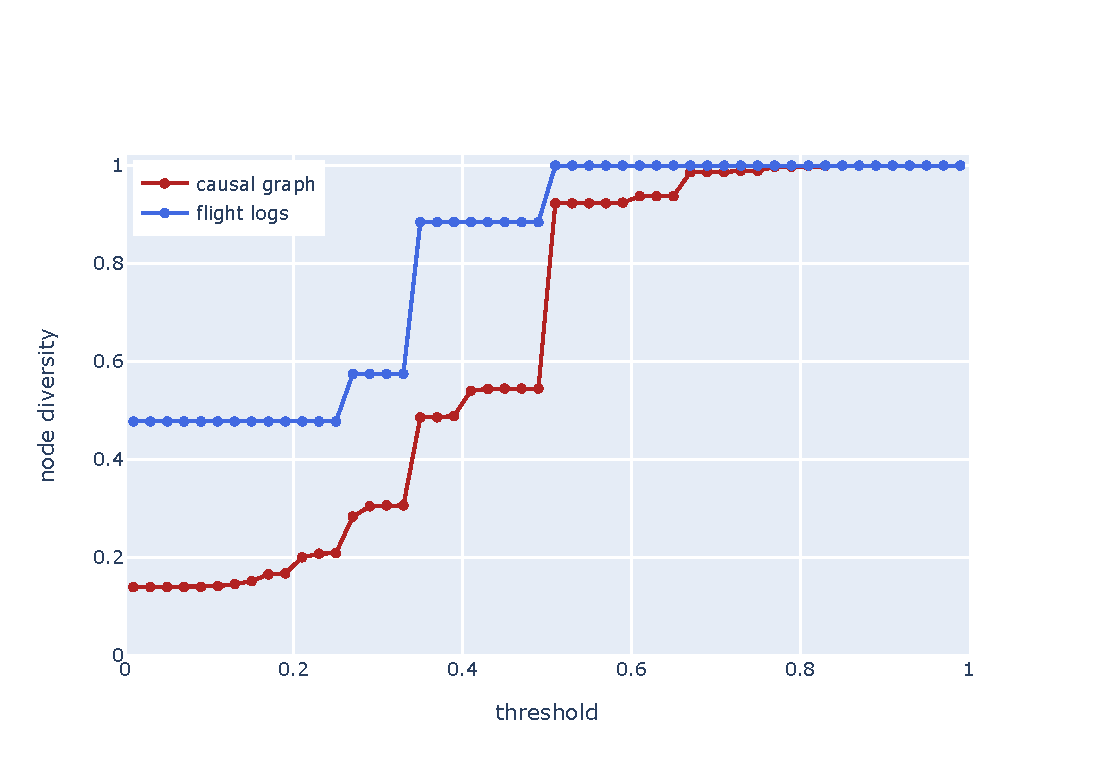
\includegraphics[scale=.65]{figures/results/node_diversity}
        \caption{Node diversity}\label{fig:node-diversity}
        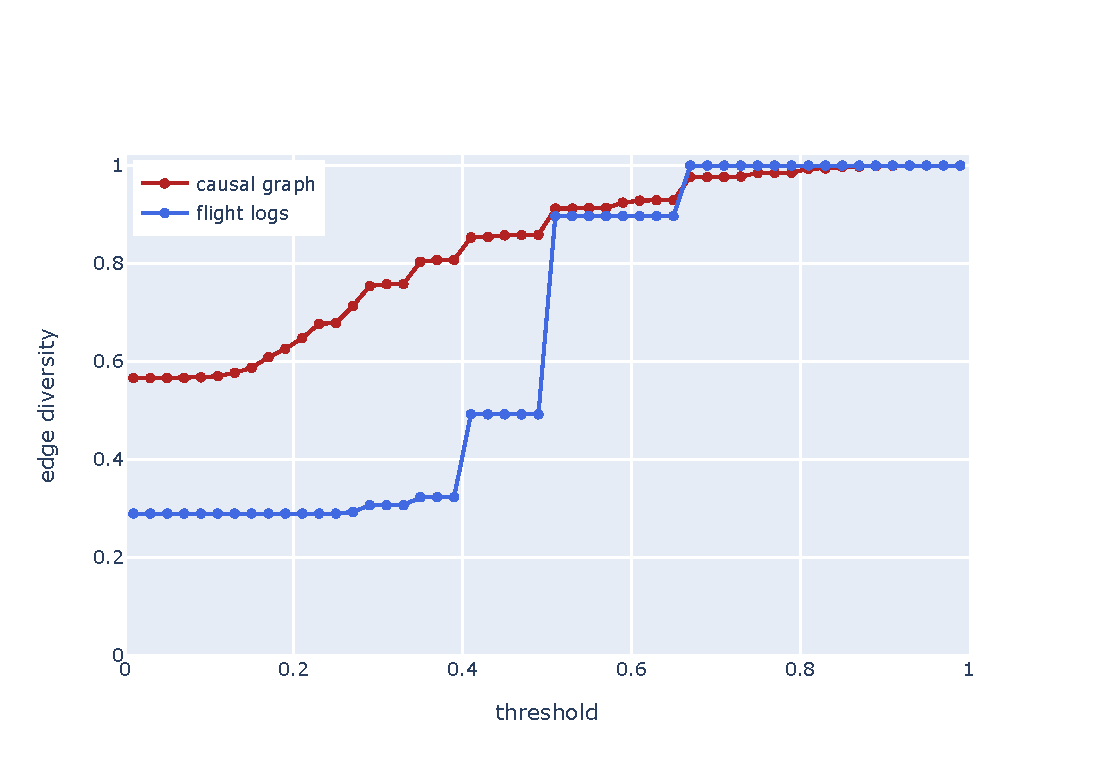
\includegraphics[scale=.65]{figures/results/edge_diversity}
        \caption{Edge Diversity}\label{fig:edge-diversity}
    \end{center}
\end{figure}
In \autoref{fig:node-diversity} we can see the diversity of the nodes from the causal graph and the flight logs.
Moreover, the diversity plot has the characteristic that it increases and converges to 1.0 (see. \autoref{subsec:diversity-of-graph}).
Furthermore, we can see that the diversity makes a vast jump around the 0.5 threshold value.
The reason for that is our similarity score (see. \autoref{eq:jaccard-similarity}).
The node similarity for the causal graph is low, which means that many nodes contain similar information.
For example, we were not able to merge the node \qq{crash}, \qq{big crash} or \qq{crash of UAV} into one node.
The flight logs have a higher diversity in comparison to the causal graph.
The diversity of nodes represents the language in the graph and describes how often the users use a similar term or phrase to describe a problem without the context of the relations.
The node diversity of the online resource is comparatively low, meaning that users use the same language or information to explain the problems.
In \autoref{fig:edge-diversity} we can see the diversity for the edges from the causal graph and the flight logs.
We can see that the edge diversity for the causal graph is higher than the node diversity because the users are more likely to express the same \ac{CEP} with different information.

\subsection{Consistency In The Online Resource}\label{subsec:consistency-question}
\begin{figure}
    \begin{center}
        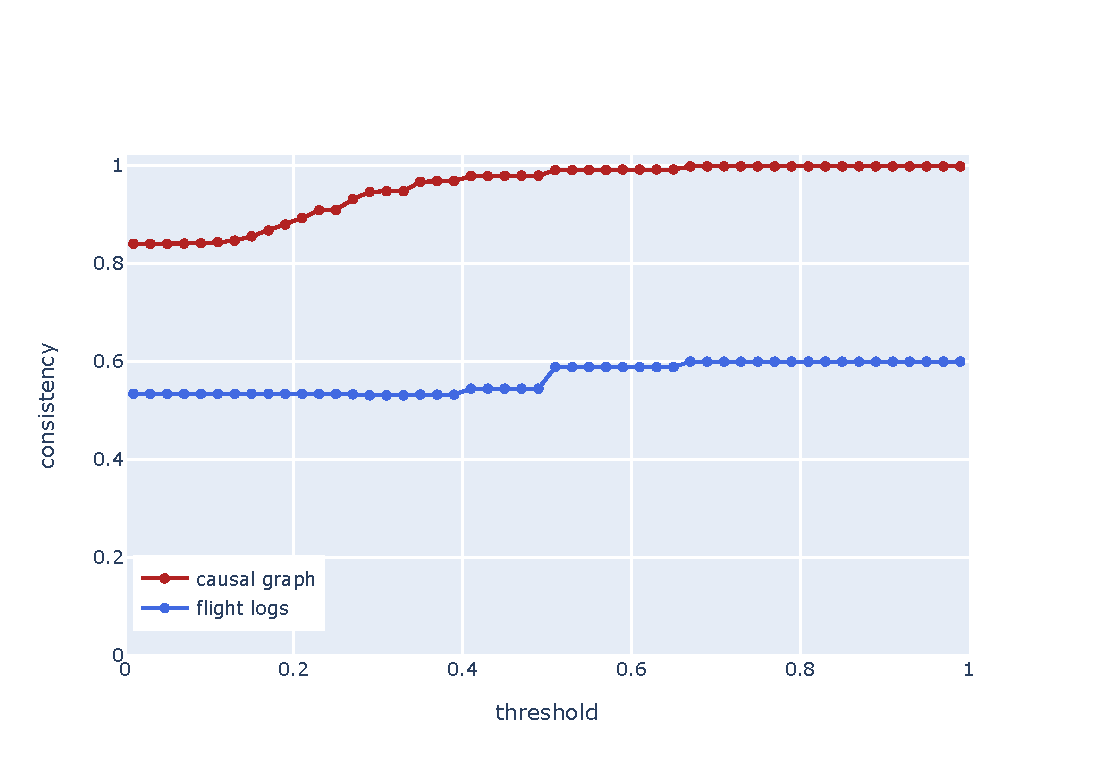
\includegraphics[scale=.65]{figures/results/consistency}
        \caption{Consistency}\label{fig:consistency}
    \end{center}
\end{figure}
In \autoref{fig:consistency} we can see the consistency plot of the causal graph and the flight logs graph.
The consistency of the causal graph is pretty high, even on a low threshold value.
Thus, we can say that the Ardupilot community is consistent in its knowledge, and the edges in the graph do not contain many contradictions.
The flight logs have a consistency score near 0.5 which means that there are a lot of \qq{ekf check} => \qq{failsafe fence} and \qq{failsafe fence} => \qq{ekf check} contradictions.
The reason for that is the way we generate the graph.
We modeled the time series data in a repeating events or errors chain.
However, building it that way was the only possible method to build a comparable graph from another resource.

\subsection{Detectability Between The Graphs}\label{subsec:coverage-question}
\begin{figure}
    \begin{center}
        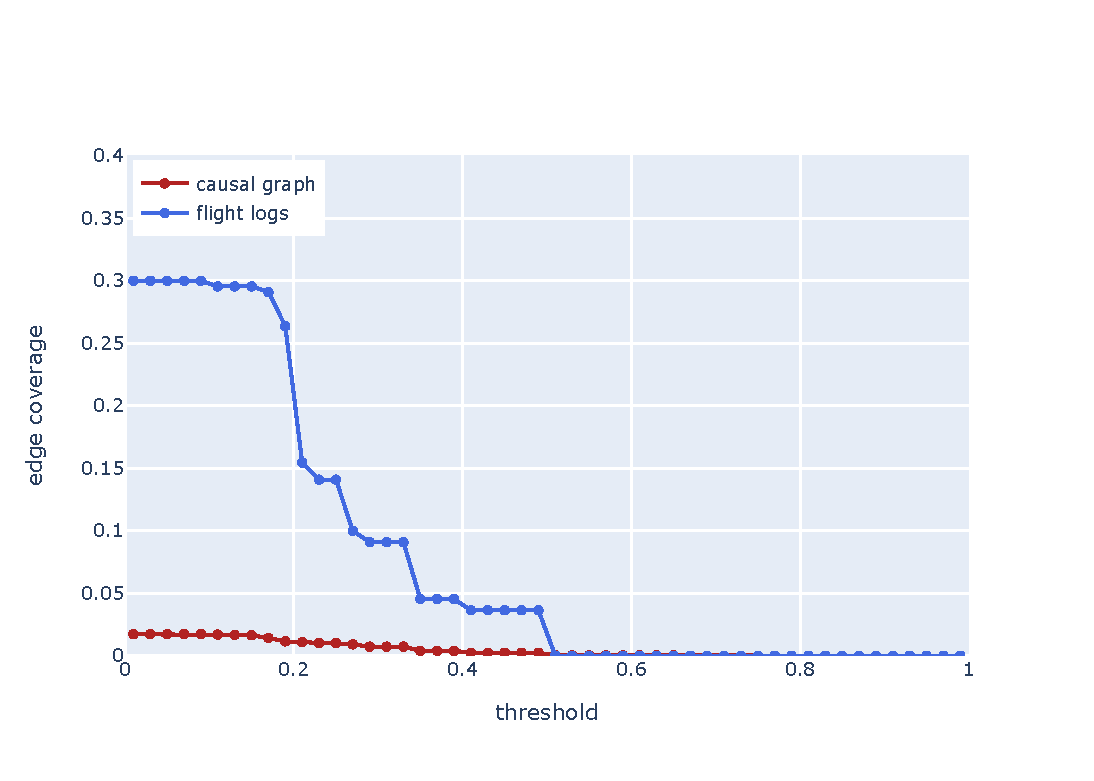
\includegraphics[scale=.65]{figures/results/edge_coverage}
        \caption{Coverage Edges}\label{fig:coverage_edge}
        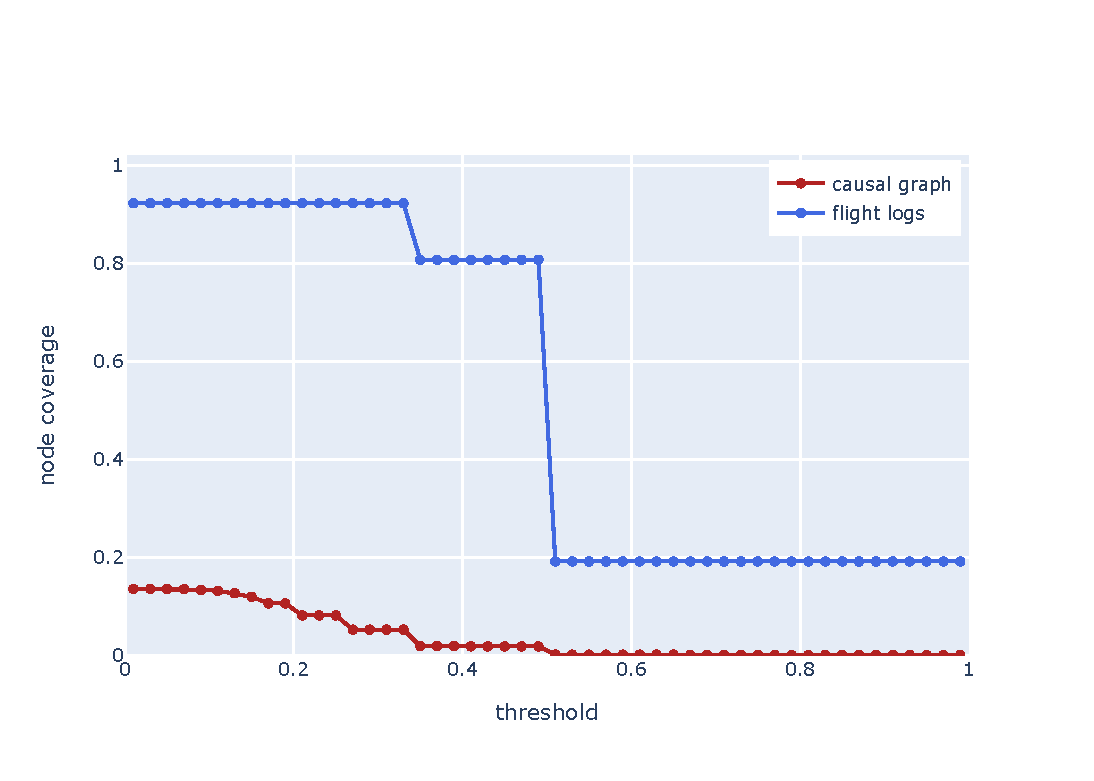
\includegraphics[scale=.65]{figures/results/node_coverage}
        \caption{Coverage Nodes}\label{fig:coverage_node}
    \end{center}
\end{figure}
In \autoref{fig:coverage_edge} and \autoref{fig:coverage_node} we can see the graph for the coverage of the nodes and edges of the causal graph and the flight logs.
The coverage for the edges of the causal graph is pretty low and only detectable on a threshold < 0.67.
The highest coverage is at the lowest threshold value, with \qq{1,73}\%.
We can first deduce that there are no exact representations of the \ac{CEP}s from the ArduPilot community and the flight logs.
Second, there are many \ac{CEP}s that the users mentioned and are not reflected in the flight logs.
This is not surprising because the flight log dataset is limited.
We can also see in the \autoref{fig:coverage_edge} figure that the coverage of the edges for the flight logs dataset is on the lowest threshold value \qq{29,6}\%.
Furthermore, we can see that the coverage score for the nodes is higher than the coverage score for the edges.
The node coverage score for the flight logs is pretty high, which means that the users mention much information that can be found in our data.

\subsection{Accuracy Of The Causal Graph}\label{subsec:accurate-question}
\begin{figure}
    \begin{center}
        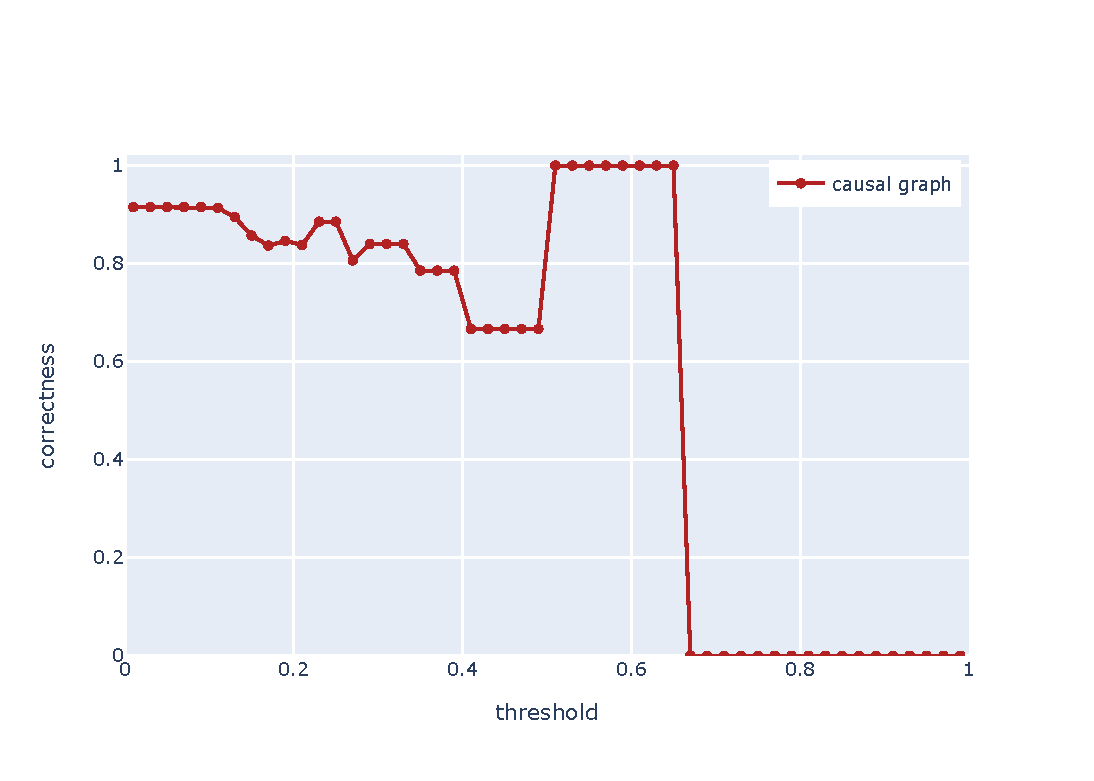
\includegraphics[scale=.65]{figures/results/correctness}
        \caption{Correctness}\label{fig:correctness}
    \end{center}
\end{figure}
The last question we want to answer is the accuracy based on the historical data.
We want to know if the graph represents correct knowledge.
Thus we need a ground truth graph to compare, like the flight logs graph.
In \autoref{subsec:coverage-question} we saw that there are few intersections between the causal graph and the flight logs.
There could be two possible reasons for that.
The first is that the knowledge of the ArduPilot community is incorrect.
The second reason could be that the ArduPilot community provides correct knowledge that is not reflected in the dataset.
We want to use the correctness score from \autoref{eq:correctness} to calculate the correctness of the domain expert knowledge graph.
Remember, the score near one indicates that a \ac{CEP} that a user mentioned is backed with the ground truth data.
In \autoref{fig:correctness} we can see the plot of the score.
The spice in the graph is correlated to the Jaccard similarity we used.
We can only calculate the correctness if there are intersections between the graphs.
Thus we do have correctness of 0 for a threshold >= 0.67 (see subsec:coverage-question).
However, the average correctness score for a threshold < 0.67 is \qq{86.51}\%.
Therefore, we can say that for the \ac{CEP}s that are reflected in the flight logs, we know that they are mostly correct.

\subsection{Mentionable Edges In The Causal Graph}\label{subsec:information-question}
\begin{table}
    \begin{center}
        \begin{tabular}[t]{||c c c c||}
            \hline
            thresh & cause                        & effect                       & info \\ [0.5ex]
            \hline\hline
            0.25   & prop motor                   & pound of thrust              & 35.027 \\ \hline
            0.25   & high vibration               & flight problem               & 32.111 \\ \hline
            0.25   & position of camara           & problem                      & 29.25  \\ \hline
            0.25   & high value                   & crosstrack problem vibration & 29.032 \\ \hline
            0.25   & combination of high altitude & problem                      & 28.488 \\ \hline
            0.25   & quad motor                   & more thrust                  & 27.000 \\ \hline
            0.25   & vibration                    & problem in gqs mode          & 26.281 \\ \hline
        \end{tabular}
        \caption{Mentionable Edges with threshold of 0.25}\label{tab:information-score-25}
        \begin{tabular}[t]{||c c c c||}
            \hline
            thresh & cause          & effect  & info \\ [0.5ex]
            \hline\hline
            0.50   & vibration      & problem & 19.000             \\ \hline
            0.50   & motor          & thrust  & 17.000             \\ \hline
            0.50   & failsafe       & rtl     & 13.000             \\ \hline
            0.50   & problem        & crash   & 11.267             \\ \hline
            0.50   & radio failsafe & rtl     & 10.000             \\ \hline
        \end{tabular}
        \caption{Mentionable Edges with threshold of 0.50}\label{tab:information-score-50}
        \begin{tabular}[t]{||c c c c||}
            \hline
            thresh & cause                            & effect                        & info \\ [0.5ex]
            \hline\hline
            0.75   & problem                          & crash                         & 7.111 \\ \hline
            0.75   & wing                             & lift                          & 6.000 \\ \hline
            0.75   & ap                               & camara                        & 5.000 \\ \hline
            0.75   & auto mode                        & kickstart acceleration        & 4.000 \\ \hline
            0.75   & certain combination of telem1 rx & boot                          & 4.000 \\ \hline
            0.75   & right step regulator             & fix output from input voltage & 4.000 \\ \hline
        \end{tabular}
        \caption{Mentionable Edges with threshold of 0.75}\label{tab:information-score-75}
    \end{center}
\end{table}

\begin{table}
    \begin{center}
        \begin{tabular}[t]{||c c c c||}
            \hline
            thresh & cause                  & effect              & info \\ [0.5ex]
            \hline\hline
            0.25   & compass problem        & crash               & 15.429 \\ \hline
            0.25   & failure of gps compass & crash               & 13.136 \\ \hline
            0.25   & short failsafe issue   & other mode          & 13.000 \\ \hline
            0.25   & gps problem            & land mode problem   & 12.000 \\ \hline
            0.25   & short failsafe issue   & mode change         & 11.077 \\ \hline
            0.25   & ekf failsafe           & change to land mode & 11.000 \\ \hline
            0.25   & gps problem            & flight problem      & 10.083 \\ \hline
        \end{tabular}
        \caption{Mentionable Edges with threshold of 0.25 and the correct label}\label{tab:information-score-25-correct}
        \begin{tabular}[t]{||c c c c||}
            \hline
            thresh & cause           & effect & info \\ [0.5ex]
            \hline\hline
            0.50   & compass problem & crash  & 10.563 \\ \hline
            0.50   & flight          & crash  & 6.000  \\ \hline
            0.50   & failsafe        & mode   & 4.000  \\ \hline
            0.50   & compass         & crash  & 3.200  \\ \hline
            0.50   & gps glitch      & ekf    & 2.000  \\ \hline
        \end{tabular}
        \caption{Mentionable Edges with threshold of 0.50 and the correct label}\label{tab:information-score-50-correct}
        \begin{tabular}[t]{||c c c c||}
            \hline
            thresh & cause & effect & info \\ [0.5ex]
            \hline\hline
            0.75   & -     & -      & -    \\ \hline
        \end{tabular}
        \caption{Mentionable Edges with threshold of 0.75 and the correct label}\label{tab:information-score-75-correct}
    \end{center}
\end{table}

We used the information score to sort all edges in descending order to find the most valuable edges in the causal graph.
In \autoref{tab:information-score-25}, \autoref{tab:information-score-50} and \autoref{tab:information-score-75} we can see such edges ranked on three different threshold values.
As we mentioned earlier, a lower threshold value allows edges that contain more information than a generic word to have a higher score which can be seen in \autoref{tab:information-score-25}.
In \autoref{tab:information-score-25-correct}, \autoref{tab:information-score-50-correct} and \autoref{tab:information-score-75-correct} we see the edges ranked by the information score.
However, we only contain edges labeled as correct regarding the flight logs dataset.


\section{Running Time Analysis}\label{sec:end-to-end-performance}
In this section, we want to analyze the overall performance of the End-o-End tool.
For computation, we used a cloud machine with 16GB RAM.
We scraped three different sources of the ArduPilot community.
We scraped 90 MB of raw textual data from the discussion forum, which took about ~17h 32min.
We scraped 9,23 MB from the discord chat in ~23 min and 11,28 MB from the documentation in ~27 min.
The scraping of the forum took that long because we needed to communicate with a web driver and wait on different actions when executing javascript.
After extracting the sentence and combining everything into one source, we found 724.922 sentences where 610.640 were from the forum, 83.577 from the discord chat, and 30.705 sentences from the documentation.
The combination and extraction of the sentences from the different sources took ~4h 12min.
We found 2758 sentences containing causation that the users explicitly mention, where 2322 of them were from the form, 200 from the documentation, and 236 from the discord chat.
We extracted the sentences in ~47min and needed ~22sec to generate the causal graph from the extractions.
It took ~3h 44min to evaluate the system for 50 different threshold values.
